\chapter{Introduction}
\label{chap:1}
\ChapterPageStuff{1}

\section{Background}\label{section:ch1_background}

Software maintenance according to the \textit{IEEE Standard 1219}\footnote{\textbf{IEEE Standards} documents are developed within the Technical Committees of the IEEE Societies, and the Standards Coordinating Committees of the IEEE Standards Board \cite{Mamone1994}.} is the process that includes the following phases \cite{Mamone1994, Hasan2012}:
\begin{itemize}
	\item Identifying the problem or modification and classification of it
	\item Analysis of the identification of the maintenance issue
	\item Design of the solution to implement maintenance
	\item Implementation of the solution
	\item System testing of the modified software system
	\item Acceptance test on the fully integrated system
	\item Delivery requirements met of the modified software system
\end{itemize}

%TODO Beter definisie vir technical debt
The maintenance problems or modifications are regularly identified and usually addressed based on an initial priority ranking. This priority ranking is determined by using classification models to determine which type of maintenance needs to be done (adaptive, corrective, perfective and preventive) \cite{Tang2010, Mamone1994, Ping2010}.\par Continuous analysis of the identified maintenance problems or modifications enables the software engineers and developers to create a preliminary plan to address these issues \cite{Port2017}. Technical debt can exist in almost every software system and should be correctly managed by analysing which maintenance issues should be prioritised \cite{DeLeon-Sigg2020, Reimanis2016}.\par Implementing a suitable maintenance framework to resolve the identified issues reduces the technical debt. Various maintenance models can be used to solve these issues when implementing any one of the maintenance types. Identifying and analysing these issues is the most challenging part of software maintenance \cite{DeLeon-Sigg2020}.

\subsection{Maintenance in software systems}
Most companies will strive to increase their digital products and services over the software project's life cycle to maximise their profits \cite{Gralha2018}. This will increase the maintenance that needs to be done on both new and old systems \cite{Niu2018, Galster2019, Hasan2012}. Although maintenance is essential for software systems, most companies do not have a defined maintenance model or process to guide them when implementing maintenance \cite{Stojanov2017}. Software maintenance is an essential task in software development, and it can directly reduce the cost and effort to create new software systems or modify them \cite{Thamburaj2017}.\par A study about software maintenance was conducted by the United States Department of Commerce. They found that the total development cost can be as much as $60\%$-$80\%$ of the total cost for the software system's development life cycle \cite{Ogheneovo2014, Stark1996, Ackermann2009, Tang2010}. These costs will increase (as shown in \Cref{fig:ch1_costsOfFixingBugs}) to maintain much older and more complex software systems, therefore implementing maintenance can keep the software system feasible in its entire life cycle \cite{Alenezi2016, Booch1986}.

\begin{figure}[!htb]
	\centering % cent the figure
	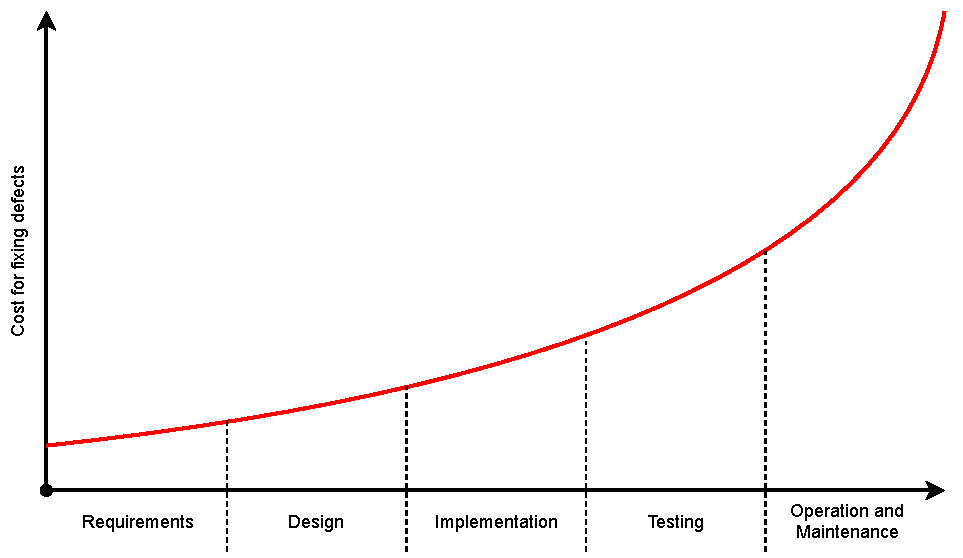
\includegraphics[width=0.5\textwidth]{Chapter1/Cost_of_fixing_bugs/Cost_of_fixing_bugs.pdf}
	\caption[Cost of fixing software system defects]
	{\textit{Cost of fixing software system defects \cite{Ogheneovo2014}}}\label{fig:ch1_costsOfFixingBugs}
\end{figure} 

Maintenance of software systems is continuous and is a reduced form of software development and is aimed to modify software systems while preserving their integrity \cite{Sneed2004, Ackermann2009, Port2017}. In \Cref{tbl:ch1_maintenanceTypes}, adaptive and perfective maintenance types are most effective when maintaining a software system's integrity. Most software engineers and developers will implement these two significant types of maintenance in their maintenance procedures.\par Adaptive and perfective maintenance ensures the software system will continue to evolve to meet the system requirements to ensure that it is useable and feasible. This is also the most effective way of reducing technical debt by adapting the software system. This continuous improvement uses about $70\%$ of the maintenance resources to manage the maintenance of the software system \cite{Kumar2013}. 

\begin{table}[!htb]
	\centering
	\caption[Software maintenance types]
	{\textit{Software maintenance types \cite{Ping2010,Hasan2012,Mamone1994}}}
	\label{tbl:ch1_maintenanceTypes}
	\begin{tabularx}{\textwidth}{|c|X|c|}
		\hline
		\textbf{Maintenance type} & \textbf{Description} & \textbf{$\%$ of maintenance activities} \\ \hline
		Adaptive & \raggedright Adaptive maintenance in software systems is any modification or enhancements to keep it usable with a changing or changed software environment. & $\approx 35.5\%$ \\ \hline
		Perfective & Perfective maintenance based are modifications made based on the change of the end-users' new requirements. It can also improve the performance or maintainability of the software system in its life cycle. & $\approx 35.5\%$ \\ \hline
		Corrective & \raggedright Corrective maintenance are improvements made to fix certain defects or errors in a software system. & $\approx 20\%$ \\ \hline
		Preventive & \raggedright  Preventive maintenance are improvements made to software systems that prevent problems in the future. & $\approx 5\%$ \\ \hline
	\end{tabularx}
\end{table}

It can be a demanding task to prioritise the available resources for certain parts of the software system to do maintenance to prevent or fix any software defects \cite{Mamone1994, Hasan2012}. The defect density can measure the software's quality in \Cref{eq:ch1_defectDensity} for a specific period \cite{Shah2012, Alenezi2016}. The defect density of a software system is the number of possible defects divided by the size of the software system.  A lower defect density indicates an improved version of the software system.

\begin{equation}
	\label{eq:ch1_defectDensity}
	Defect~Density = \frac{CNDD}{KLoC},
\end{equation}

where:

\begin{itemize}
	\item $CNDD$ is the cumulative number of defects in the post-release version of the software system
	\item $KLoC$ (thousands of lines of code) is the size of the observed executable code in a software system 
\end{itemize}

In open-source software systems, the defect density increases due to the number of developers working on the same software system and the size of the system itself \cite{Rahmani2010}. Adding more developers to improve a software system may not always have an improvement in each of the maintenance types in \Cref{tbl:ch1_maintenanceTypes}. There might be even a need to increase the corrective maintenance efforts as more developers are already trying to resolve the existing maintenance issues.\par The size of the software system in OSS does have an impact on the defective density \cite{Rahmani2010}. Naturally larger and more complex software systems will have larger defect density as the system will be complex and some parts of it will be older than others \cite{SourceForged2009}. 

In \Cref{fig:ch1_costsOfFixingBugs}, the cost of maintenance increases if the maintenance activities increase when implementing the four major types of software maintenance. These maintenance activities cannot be neglected as the software will most likely keep evolving as new features are added to keep it useable \cite{Alenezi2016}. \par In an ideal situation, the maintenance should be done during the software development planning phase. Due to time constraints and available resources, it is not easy to plan any maintenance phase for most software engineers and programmers. The cost increases of maintenance due to a lack of planning or preventive measures to keep the quality software from degrading \cite{Alenezi2016}.

\subsection{Problems with implementing software maintenance}\label{sec:ch1_maintenanceProblems}

Under most circumstances, maintenance is implemented if a software system does not meet the required functions specified by the performance requirements \cite{Ogheneovo2014, Sneed2004}. These systems will also most likely have multiple software defects or will be extremely complex due to:

\begin{itemize}
	\item \textbf{Problem domain being complex:} The software may not be well defined or structured. This is due to how large the software systems grow over their entire life cycle or duplicate software components that are made. This is caused by poor understanding of the system architecture by developers not doing the required maintenance on these systems and just adding new features \cite{Galster2019, Booch1986}.
	\item \textbf{Difficulties of managing development process:} Most companies will strive to increase their digital products and services over the life cycle of the software project to maximise possible profits with the resources invested \cite{Niu2018}. Increasing production of the development process will only strain the maintenance software systems \cite{Sneed2004}.\par The development team needs to prioritise concrete tasks in the development process to make the project feasible by focusing on these tasks can lead to poor decisions being made about the required task to perform software maintenance \cite{Galster2019, Ogheneovo2014, Lenarduzzi2017}. 
	\item \textbf{Flexibility of the software:} Trying to predict what the possible future architecture may look like and modifying it while preserving the software's integrity may be difficult in software maintenance \cite{Garlan1999}. Software is flexible if it is adaptable to the problem domain when adding modifications to it \cite{Ogheneovo2014}.\par Most development teams will follow a software development methodology to create a future architecture that is modular and structured to preserve the development integrity of new software \cite{Vijayasarathy2016, Rehman2018}. This will also have an impact on the type of maintenance activity (as in \Cref{tbl:ch1_maintenanceTypes}) the development team will use, which are called corrective, perfective, adaptive and preventive maintenance \cite{Thamburaj2017, Hasan2012, Stojanov2017, Snipes2018}.
	\item \textbf{Change in user's requirements:} In software development, the users will often request new additional requirements to the software systems delivered to them \cite{Ogheneovo2014}. Modifying software systems may include new and additional features that change the initial system architecture. Maintenance of these systems is crucial to ensure that existing components of the system will work as intended with the new components that are added.
\end{itemize}

%TODO hier is waar need of study moet begin 
%TODO What is the problems with What is the problem with event logging
%TODO How can analysis improve maintenance
\clearpage

\section{Event logging}\label{sec:ch1_eventLogging}
Event logging is a proven implementation to get information about the behaviour of software systems \cite{Baccanico2014}. An event log $W$ is the sequence of log entries of events $E$ or a multi-set of traces when $T$ is a finite set of defined tasks being done and $T^+$ is a set of all the non-empty finite sequences of $T$ \cite{Kherbouche2017}

\begin{equation}
	\label{eq:LogEvent}
	W = (E, C, A, \partial, \wp, \Gamma, \succ) \subseteq T^+,
\end{equation}

where:

\begin{itemize}
	\item $E$ is a finite set of events,
	\item $C$ is a finite set of cases,
	\item $A$ is the finite set of additional data that can be split up into disjoint sets of event attributes (timestamps $T_S$, cost $O$, resources $R$, event types, $E_T$ and data elements $D$),
	\item $\partial$ is the \textit{surjective}\footnote{\label{ftn:Surjective}A \textbf{surjective} function is a way of matching the members of a set $A$ to a set $B$ \cite{Szendrei1990}.} $E\rightarrow C$,
	\item $\wp$ is the \textit{surjective}\footref{ftn:Surjective} $A\rightarrow E$,
	\item $\Gamma$ is the \textit{surjective}\footref{ftn:Surjective} $E\rightarrow T$,
	\item $\succ \subseteq E\times E$ is the total ordered events in $E$ that belongs to a specific case that is called a trace.
\end{itemize}


Event logging has three major purposes that are divided into other major industry implementations in \Cref{tbl:ch1_eventLogsUsage} \cite{Pecchia2015}:

\begin{itemize}
	\item \textbf{state dump} which is reporting of values of certain variables or data structures inside the software system.
	\item \textbf{execution tracing} is the reporting of certain states of the software system or what is currently happening in the software system,
	\item \textbf{event reporting} which focuses on any desired events in the software system that has textual information of that event.
\end{itemize}

As mentioned in \Cref{section:ch1_background}, software maintenance can make use of event logs to improve software maintenance. It is a common practice in the software industry to record any detailed system run-time information into logs to be analysed later by developers or software engineers to solve software-related problems with the system as in \Cref{tbl:ch1_eventLogsUsage} \cite{Zhu2019}.\par The technique to collect numeric or textual data that describes the behaviour of a computer system is called event logging \cite{Pecchia2015, Baccanico2014}. Event logs are collected textual data containing the records of events that happened in a software system and are used for system management tasks as in \Cref{tbl:ch1_eventLogsUsage} \cite{Rong2018a, Rong2018, Baccanico2014}.

\begin{table}[!htb]
	\centering
	\caption[Event logs usage]
	{\textit{Event logs usage}}
	\label{tbl:ch1_eventLogsUsage}
	\begin{tabularx}{\textwidth}{|l|X|}
		\hline \textbf{Usage} & \textbf{Description} \\
		\hline Debugging of software systems and services & Event logging is mostly used to record events or behaviours of software systems or services during its runtime \cite{Rong2018a}.\\
		\hline Anomaly detection & Event logs can be used to detect any abnormal system behaviour using an anomalous detection algorithm using logging data \cite{Gurumdimma2016}. This can also be used to find any potential vulnerabilities or defect prediction in the software environment \cite{Dwyer2013}. \\
		\hline Performance diagnosis & Software performance is important to producing quality software for the end user \cite{EvangelinGeetha2007, Baccanico2014}. This is also important to make informed decisions on how to improve the software system or service for improved performance and other resource and financial implications.\par This type of performance event logs of the software systems or services are used to monitor the software system, which is useful for resource tuning, load balancing and checking system scalability in the entire life cycle of the software system or service \cite{Song2017}. \\ 
		\hline Auditing & In a software environment there can be significant changes to the database data that might need to log for auditing purposes \cite{Rong2018a}. All establishments and enterprises need to ensure that compliance with the industry regulations is met with their software systems by adding audit logs. They are also legally bound to have audit logs to provide legal evidence for any legal investigation or administrative tasks to ensure that accountability is maintained. \\
		\hline Error and failure analysis & Event logs are used to analyse the failure behaviours of software systems which enable software engineers or developers to understand the failure modes of the system, find the root cause of these failures, prevent them and improve the reliability of the future releases of the system \cite{Cinque2013}.\\
		\hline Analysis of security alerts & In any software environment or information technology infrastructure, security is a major concern for any organisation \cite{Pathan2014, Dwyer2013}. It is important to know the overall security status of the software system. \\
		\hline
	\end{tabularx}
\end{table}

\clearpage

\subsection{Logging practice in software development}
Logging practice in software development is not always well documented and can there be multiple implementations of different logging mechanisms in the same software system \cite{Pecchia2015, Kitchenham2007}. In modern software systems, the logging practice is a crucial part of the development of software and the maintenance of it in its entire life cycle \cite{Rong2018}.

\subsubsection{Logging practice guidelines}
In \Cref{apx:loggingPractice} there has been a rise of new studies that focus on providing suitable logging practice guidelines to software engineers and developers. Logging in the industry makes use of many third-party logging libraries and frameworks such as Apache's log4net and Microsoft's ULS frameworks \cite{Zhu2015, Rong2018}.\par Software engineers and developers can use these tools to implement logging in a compatible software system. They will still need to know how to strategically place the logging points so that the desired logs can be obtained. Using guides provided by the tools and other online guides, the logging practice can be implemented When using a third-party logging mechanism the software engineers and developers will in most cases need to:

\begin{itemize}
	\item add the logging points in the software system at locations where it can capture the desired logs,
	\item enables the log parsing stage to write a log entry into a database.
\end{itemize}

Logging guides can give examples and suggestions on where to place the logging points but that can still be sometimes difficult for software engineers and developers to identify these desired locations. This can be difficult due to logging guides being mostly application-specific or the logging mechanism can only capture certain event types to create event logs. \par For more custom logging the software engineers and developers will need to create new logging mechanisms. This adds new requirements for the logging mechanism to be functional. For a logging practice to be successful two important problems need to be resolved \cite{Zhu2015, Zhu2019, Rong2018}:

\begin{itemize}
	\item What needs to be logged?
	\item Where to log?
\end{itemize}

\subsubsection{What needs to be logged?}
In \Cref{tbl:ch1_eventLogsUsage} the use of logging is diverse and will have an impact on how the logging mechanism will be designed. In this study, the purpose of the logs is to be used for user-based activity tracking, therefore what needs to be logged should be focussed on user-based events. The requirements for a user-based event should be defined and a log attribute model can be designed for those requirements.

\subsubsection{Where to log?}
Different types of logs will only be present in the software system at certain locations during runtime. Knowing what to log narrows down which locations can be used to obtain certain events while they are present.

\clearpage

\subsection{Logging quality}\label{sec:ch1_loggingQuality}

Software engineers and developers will need to make informed logging decisions to cover the necessary run-time information without negatively impacting the software system's performance \cite{Zhu2015, Zhu2019, Kherbouche2017}. An event log quality model in \Cref{fig:EventQModel} can be used define to ensure that the event logs will have consistent integrity when capturing the event log data. The event log quality model in \Cref{fig:EventQModel} consists of four different levels to define each property of the event log model:

\begin{itemize}
	\item Root level for the event log quality model,
	\item Dimension level which consists of four main dimensions of the event log quality model according to \cite{Kherbouche2017} (complexity, accuracy, consistency and completeness of the event log),
	\item Attributes level where a set of quality attributes for the dimension level,
	\item Measurement level which should be defined in the design process of the logging mechanism to achieve the attributes and dimension levels.
\end{itemize}

\begin{figure}[!htb] % An h :here, t: top, b: bottom.
	\centering % cent the figure
	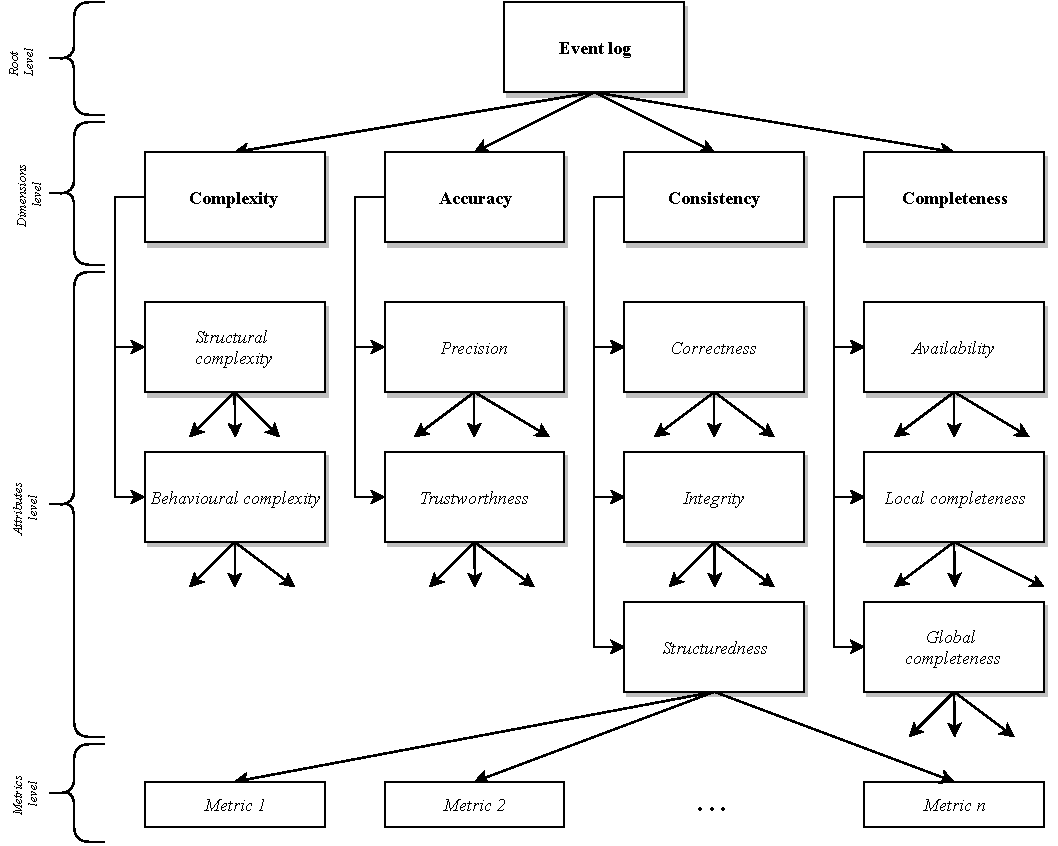
\includegraphics[width=0.9\textwidth]{Chapter1/Event_Log_Model/Event_Log_Model.pdf}
	\caption[The event log quality model]
	{\textit{The event log quality model \cite{Kherbouche2017}}} \label{fig:EventQModel}
\end{figure}

\subsubsection{Accuracy of event logging} 
It can become difficult to log every event in a software system as these systems will get larger and more complex during their development life cycle \cite{Stojanov2017}. Precisely capturing certain events that need to be logged needs to be consistent to ensure that the data is trustworthy and reliable to use. The log attributes (\Cref{tbl:ch1_logBasicAttributes}) of the event log also need to be precisely captured for each event log and should be correct.\par Capturing more event logs doesn't guarantee that the accuracy of the event log is on an acceptable level as the log's attributes can be incorrect or cause duplicated events logs if the data is the same in a sequence of event logs. In \Cref{tbl:ch1_loggingTooMuch} is the common problems associated with too much logging. \par The accuracy and trustworthiness of the event log are more important than capturing a large number of available event logs in a software system \cite{Zhu2015, Jans2012}. The extra unnecessary logs will also take up more storage space store which will increase costs and possibly the performance of the software system. 

\begin{table}[!htb]
	\centering
	\caption[Problems with too much logging]
	{\textit{Problems with too much logging \cite{Zhu2015}}}
	\label{tbl:ch1_loggingTooMuch}
	\begin{tabularx}{\textwidth}{|l|X|}
		\hline \textbf{Problem}  & \textbf{Description} \\
		\hline \textbf{Excess code} & Adding multiple logging points may increase the amount of code added to the software system to capture the event logs. The code may take some time to write and maintain. This can increase the structural and behavioural complexity of the code in its entire life cycle. \\
		\hline \textbf{System resource impact} & With the additional code needed to capture the logs the system resource usage such as the CPU and I/O channels will increase. This may negatively impact the performance of existing system operations or increase the cost to keep the system at the same operation speed by increasing the system resources.\\
		\hline \textbf{Unusable logs} & Adding numerous logging points or logging too much at points can produce numerous trivial or useless logs that will not improve the system utilisation analysis. When implementing the system utilisation analysis stage the logs might need to get filtered more or modified to be more meaningful. More event logs can have missing or incomplete logging attributes due to the excessive logging points that have been added. The increase in the behavioural complexity of the log can impact the decisions that are made to improve software maintenance. \\
		\hline
	\end{tabularx}
\end{table}

\subsubsection{Event log complexities}
Software always has some complexity involved and it will always increase when the software system becomes larger. For the event log quality model the complexity of the event can be split into two different complexities which are \cite{Kherbouche2017}:

\begin{itemize}
	\item Structural complexity is the application of different algorithms in the software which allows the event log to be evaluated when it occurs which can alter the behaviour of the event log.
	\item Behavioural complexity in event logging is the complexity of the behaviour of the event logs that refers to the number of smaller events in each captured trace and the different variations of these traces within an event log.
\end{itemize}

These two complexity attributes can be costly when the event logging mechanism needs to be constantly maintained in large software systems where it can impact the rest of the system's performance or integrity of the captured event logs \cite{Ogheneovo2014}. The constant modification of the event log software can be due to technical debt as the event log system's complexities lead to technical issues when attempting to log an event or is not compatible with other systems \cite{DeLeon-Sigg2020}.  

\subsubsection{Consistency of event logging} 
The event logs' accuracy and consistency are critical when making reliable decisions based on the identified behaviour of the software system with the historical data that exists in the event logs that is discussed in the previous event log quality dimension \cite{Stojanov2017, Kherbouche2017}. With the accuracy and trustworthiness of the event logs correctly applied, the consistency of the event logs should be on an acceptable level to be correct and verifiable when comparing it to the software system. \par An event log quality model is essential to ensure that the logs will be of high quality for the data mining process in \Cref{sec:ch1_systemUtilisation} and therefore the event log data should be consistent. To ensure the consistency of the event logs the structure of the event logging points and log parsers (\Cref{sec:ch1_loggignPoints}) should be consistent to capture all the important log attributes. The event log data should also be consistently analysed with different methods used on it as part of the consistency of the event logging process.

\subsubsection{Completeness of event logging} 
The event logs will be analysed at a later stage, the logs should be fully complete when it is being used as some of the other logging attributes might not be available at that stage. The event logs' available attributes should be accurately captured before attempting to store them in a database to ensure that there is no missing event data or missing events if the event is discarded due to it being incomplete. There are two types of completeness attributes excluding the availability attribute in the \Cref{fig:EventQModel}:

\begin{itemize}
	\item Local completeness refers to all event data that can be captured for an instance of the event taking place that can be added as a log attribute to the event log \cite{Kherbouche2017, VanDerAalst2004}.
	\item Global completeness refers to the occurrence of all possible outcomes or behaviours of the event logs that can be captured which is required for the system utilisation analysis \cite{Kherbouche2017, VanDerAalst2004}.
\end{itemize}

Ensuring that both completeness levels are achieved and that the event log data is complete can impact performance if certain data is not directly available during the instance when the event has occurred. The logging mechanism needs to capture this as efficiently as possible without causing performance issues to the rest of the software system's operations \cite{Zhu2015, Zhu2019}. 

\subsection{Logging parsing and log points}\label{sec:ch1_loggignPoints}
Knowing what to log can significantly reduce any overhead the logging mechanism may produce in the software system \cite{Jia2018, Pecchia2015}. Preserving quality (as described in \Cref{sec:ch1_loggingQuality}) is a necessity to ensure that the logs that are obtained will fulfil their purpose when analysing it.

\subsubsection{Logging attributes}
Before the logs can be parsed to a structured dataset the key attributes need to be defined that will describe the event log \cite{Bekeneva2020}. The attributes in describing in \Cref{tbl:ch1_logBasicAttributes} are the most basic attributes a log event should have. They make it possible to mine and analyse the logs based on their attributes and increase the precision and reliability of the event log \cite{Kherbouche2017}.

\begin{table}[!htb]
	\centering
	\caption[Basic log event attributes]
	{\textit{Basic log event attributes \cite{Bekeneva2020}}}
	\label{tbl:ch1_logBasicAttributes}
	\begin{tabularx}{\textwidth}{|c|X|}
		\hline \textbf{Attribute} & \textbf{Description} \\
		\hline Case number & Unique identifiers for each log event. This is usually the primary identifier for the log event. \\
		\hline Timestamp & The time and date that the log event occurred. This is part of identifying the order of events or traces along with the case number of the event log \cite{Kherbouche2017}. \\
		\hline Event type & Each log event can be grouped with other log events that have similar actions that happened. These event-type attribute needs to be classified based on a state change, failure to execute an instruction, or due to an occurrence of activity like the availability of a service \cite{Fedaghi2010}. \\
		\hline Resource & These sources from which the event took place. This can be parts of the software that performs the event action or was the cause for the event to be initiated by another part of the software. \\
		\hline Other metadata & This is any other relevant information that can be used as the event log's attribute that further expand the information of the log event. This can be one extra field or many other individual attribute fields.\\
		\hline
	\end{tabularx}
\end{table}

The case number and timestamp attributes in \Cref{tbl:ch1_logBasicAttributes} can be defined anytime during the logging process. This is not the case for the rest of the attributes. Every log should have a defined action that will put it in a group of logs that can be defined as the event type. These event types can be either predefined of what is expected from the event action or will need to be observed later analysis of the logs in case there is no clear grouping of the logs \cite{Bekeneva2020, Fedaghi2010}.

\subsubsection{Log points}

The sources of the log event assist on determine the location where the event took place. For event logs this essential to try to recreate scenarios or actions based on the relevant parts of the software system that participated in the event action.\par Other metadata can increase the log quality by providing additional information about software instructions that were executed. These attributes add more information that can be used to recreate the scenario or action that may be unique parameters or other events that participated in the event log.\par To get the attributes in \Cref{tbl:ch1_logBasicAttributes} an instruction generates the log and parses it onto a data set. These log instructions are called logging points in the software environment \cite{Pecchia2015, Zhu2015}. They can be any instruction such as a print function that displays the information for the user to more complex functions or libraries that can be created by third-party developers.

In \Cref{fig:ch1_logParsing} is an example of a logging point parsing a log message in a structured log. The defined attributes are captured by the logging point when the event takes place or occurred. The created log message is then parsed into a structured log to be safe in a database or displayed. The logging point should be strategically placed to capture the required attributes to complete the log event \cite{Fedaghi2010}.

\begin{figure}[!htb]
	\centering % cent the figure
	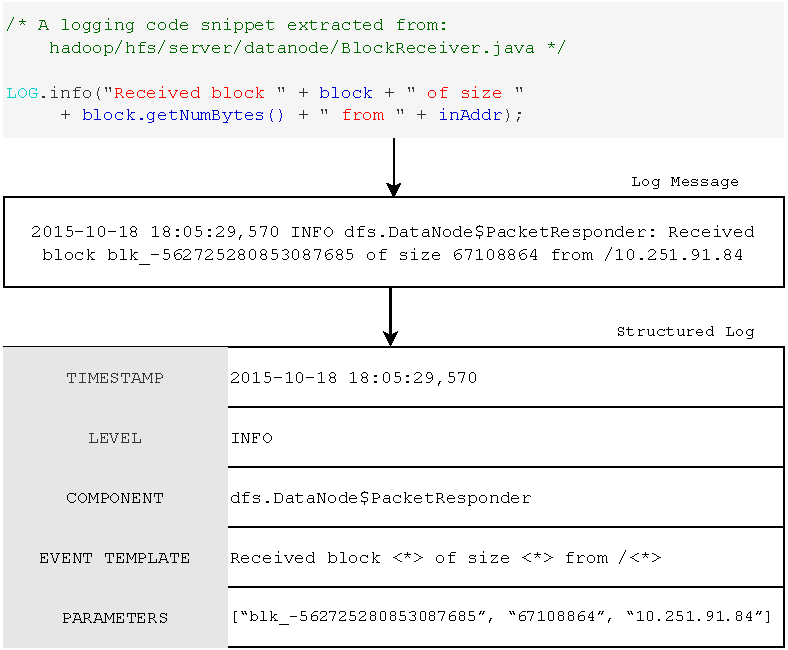
\includegraphics[width=0.9\textwidth]{Chapter1/Log_Parsing_Example/Log_Parsing_Example.pdf}
	\caption[An illustrative example of log parsing]
	{\textit{An illustrative example of log parsing \cite{Zhu2019}}} \label{fig:ch1_logParsing}
\end{figure}

Determine where to place the logging point in a giving software is directly impacted by what the attributes are and if the captured log will be of high quality as described in \Cref{sec:ch1_loggingQuality}. The availability of consistent high-quality logs will directly impact the process mining in the analysis of the logs \cite{Kherbouche2017}.\par To strategically place a logging point developers needs to consider what the activation of the logging point will be during the runtime of the software system \cite{Pecchia2015, Cinque2013}. The activations can be simple if a statement meets certain criteria or instructions that execute after when an event or action took place (e.g. runtime errors). \par In this case for a user-based activity log the activation points should be when the user interacts with the system through a graphical interface to perform a certain task. This action can be seen as a user-generated event and the logging points can be placed at strategic areas of the system code to capture the event taking place. 

\clearpage

\section{System utilisation analysis}\label{sec:ch1_systemUtilisation}
In Web-based applications, the process to get usage statistics and user behaviour data is called Web analytics \cite{Kocsis2012}. Web analytics can be used for user modelling efforts. User modelling in software engineering is the customisation and adaptation of the software systems to the users' required needs \cite{Waqar2017, Paliouras1999}. \par Web analytics focuses on different analytics in \Cref{tbl:ch1_webAnalytics} for the analysis. These same analytics can be used for none Web-based applications as the: 

\begin{itemize}
	\item identity of the user can be captured if the software system uses a software license,
	\item different parts of the system can be tracked.
\end{itemize} 

\begin{table}[!htb]
	\centering
	\caption[Web analytics for user-based data]
	{\textit{Web analytics for user-based data}}
	\label{tbl:ch1_webAnalytics}
	\begin{tabularx}{\textwidth}{|l|X|}
		\hline \textbf{Analytics}  & \textbf{Description} \\
		\hline \textbf{Identity of the user} & This is any information about the user's identity in the software system. Users can have different roles when using the software system such as a system admin or general user. These roles mostly dictated what the user can access and do on a website. \\
		\hline \textbf{Site interaction} & The different Web sites the user is accessing during their active Web session. This would also contain all the information about: 
		\begin{itemize}
			\item how often the users visit a website,
			\item how much time they spent on a specific website,
			\item navigation between different web pages of the website.
		\end{itemize}
		\\
		\hline
	\end{tabularx}
\end{table}

As previously stated that the logging mechanism is used to obtain the user-based event logs and system utilisation analysis will need to focus on th

\clearpage

\section{State of the Art}
In \Cref{section:ch1_background} the importance of software maintenance is discussed in the background and that system utilisation is needed to assist with the software maintenance efforts.

\subsection{State of the art summary}

\begin{table}[!htb]
	\centering
	\caption[State of the Art]
	{\textit{State of the Art}}
	\label{tbl:CH1_StateOfTheART}
	\begin{tabularx}{\textwidth}{|c|Y|Y|Y|Y|Y|}
		\hline \textbf{Ref.} & \RaggedRight \textbf{Log activity types} & \RaggedRight \textbf{Log attributes} & \RaggedRight \textbf{Logging points} & \RaggedRight \textbf{Log extraction and visualisation} & \textbf{System utilisation analysis} \\
		\hline 1 & 2 & 3 & 4 &  5 & 6 \\
		\hline \cite{Zhu2015} & \cmark & \cmark & \cmark & \xmark & \xmark \\
		\hline \cite{Bekeneva2020} & \cmark & \cmark & \cmark & \cmark  & \cmark \\
		\hline \cite{Pecchia2015} & \xmark & \xmark & \xmark & \cmark & \cmark \\
		\hline \cite{Kocsis2012} & \xmark & \xmark & \xmark & \cmark & \cmark \\
		\hline \cite{Kherbouche2017} & \xmark & \xmark & \xmark & \cmark & \cmark \\
		\hline
	\end{tabularx}
\end{table}


\clearpage

\section{Problem statement}
Software maintenance is a vital part of the entire life cycle of any software system. Implementing maintenance on software systems is most effective if it's done on systems that are utilised more by users. Some of these systems may also not be in use anymore and can be deprecated to improve system quality and remove unused code to not waste any resources to maintain and run it.\par A possible solution to this problem is using event logging to determine the utilisation of the system as it is a proven method industry to track system utilisation usage. Developers have access to third-party software logging tools to get the event logs. Most of the tools focus more on system runtime utilisation than user activities. There exist logging tools that can track user-based activities depending on the framework the software system is developed on.\par Developers still need to design the overall logging mechanism and decide where to place the logging points to capture the event logs in a software system. There are proven methods to create a suitable logging mechanism but not all of them include the analysis of the logs for user-based utilisation.

\section{Objectives of the study}
This study aims to develop a logging mechanism to track user-based activities to perform an analysis of these logs to improve system maintenance in a software environment. The study is divided into two components to achieve the primary goal, which is the design and implementation of the logging mechanism and the analysis of the system utilisation to improve system maintenance to improve software maintenance.

\subsection{Logging mechanism:}
\begin{itemize}
	\item Random text.
\end{itemize}

\subsection{Analysis of the system utilisation to improve software maintenance}
\begin{itemize}
	\item Random text.
\end{itemize}

\section{Overview of the dissertation}
\subsubsection{Chapter 1: Introduction}
This chapter contains the background of software maintenance and system utilisation analysis. It defines the complexities and general issues with software maintenance when implementing it and not implementing it.

\subsubsection{Chapter 2: Methodology}
This chapter contains the design of the generic method used to create a logging mechanism from a set of defined logging points and log attributes. The second part of this chapter is the system utilisation analysis by using the captured logs to create an analysis report.

\subsubsection{Chapter 3: Results}
This chapter contains the 
